\documentclass[11pt]{report}

% Math
\usepackage{amsmath}
\usepackage{amssymb}
\usepackage{braket}

% Figures
\usepackage{graphicx}
\usepackage{caption}
\usepackage{ragged2e}

% Better typography
\usepackage{microtype}
\usepackage[T1]{fontenc}
\usepackage{lmodern}

% Links and equation references
\usepackage[colorlinks=true,
            linkcolor=blue,
            citecolor=blue,
            urlcolor=blue]{hyperref}

\begin{document}




\chapter{Rydberg excitations}
\label{rydberg}

Quantum entanglement -- the non-local correlation between particles such that the system state cannot be factorized into individual single-particle states -- is the fundamental resource enabling quantum computational advantage~\cite{Jozsa2003}. It is the primary reason why quantum many-body systems are hard to simulate classically and the mechanism through which quantum algorithms outperform their classical counterparts. In neutral atom arrays, high-fidelity entanglement is typically generated via Rydberg interactions, leveraging the strong interactions between atoms excited to high-principal-quantum-number ($n$) electronic orbits \cite{Jaksch2000, Levine2018, Evered2023, Tsai2025}. This chapter describes the preliminary progress of this platform on Rydberg physics, providing the foundational framework for high-fidelity entanglement generation currently being pursued by the next generation of researchers in the laboratory.

\section{Rydberg Laser System: General Overview}
\label{sec:RydbergLaser}

The current version of the experiment utilizes a two-photon excitation scheme to Rydberg state (Figure~\ref{fig:rydberg_general}a), similar to the first generation atom array platform within our group \cite{Evered2023}. The two lasers (at 420 nm and 1015 nm respectively) couple the $5\text{S}_{1/2}$ hyperfine clock qubit $\ket{1}$ state ($\ket{F=2, m_F=0}$) to the $53\text{S}_{1/2}$ Rydberg state via the intermediate $6\text{P}_{3/2}$ state. The 420-nm laser is $\sim$7-GHz red detuned from the $6\text{P}_{3/2}$ state. 

\begin{figure}[h!]
\centering
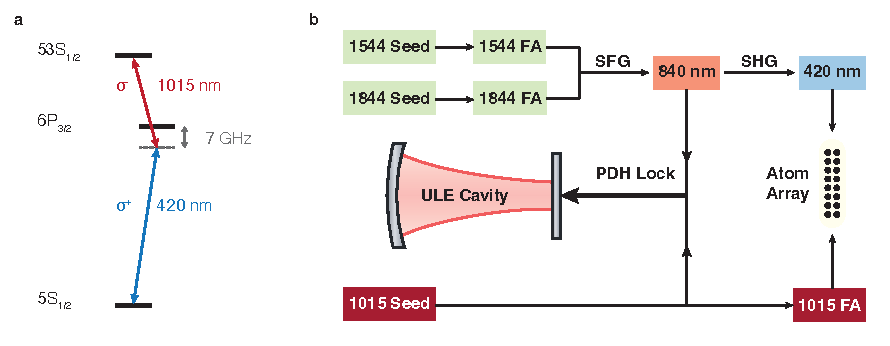
\includegraphics[width=1.0\textwidth]{figures/rydberg/rydberg_general.pdf}
    \caption{\justifying
    \textbf{Rydberg excitation scheme. a,} We employ a $\sigma^+ - \sigma^-$ two-photon excitation scheme to $53\text{S}_{1/2}$ Rydberg state via $6\text{P}_{3/2}$ intermediate state. Intermediate state detuning is currently 7~GHz. \textbf{b,} The laser exciting the first leg of the two-photon transition is a 420-nm laser frequency doubled from an 840-nm laser. The 840-nm laser is the output of sum frequency generation between a 1544-nm fiber amplifier and a 1844-nm fiber amplifier. $\sim$ 1-mW of power is sampled from the 840-nm laser and coupled to a ULE cavity for PDH locking of the laser's frequency. The laser exciting the second leg of the two-photon transition is a 1015-nm fiber amplifier laser. A sample of the 1015-nm seed laser is also coupled to the ULE cavity for frequency locking (PDH lock).
    }
\label{fig:rydberg_general}
\end{figure}

A summary description of the Rydberg laser system is shown in Figure~\ref{fig:rydberg_general}b. The 420-nm laser is frequency doubled from an 840-nm Precilaser fiber laser, which is generated by sum frequency generation of a 1544-nm fiber amplifier and a 1844-nm fiber amplifier. The seed lasers are a 1544-nm fixed external cavity diode laser (FECL) and a 1844-nm fiber distributed-feedback (DFB) laser, both supplied by Precilaser. The non-linear crystal used for frequency doubling is LBO~\cite{Velsko1991}, and it is placed inside a bow-tie cavity (Agile Optic) to benefit from cavity power buildup~\cite{Hannig2018}. Our Precilaser 840-nm system outputs 6 W of optical power, and we get $2\sim3$ W (crystal may have degraded over time) of 420-nm power after the resonant second harmonic generation (SHG). Recent laser developments have already made possible 10-W 420-nm laser solutions (doubling from 30-W 840-nm fiber laser), so the Rabi frequency of the lower leg transition can certainly be improved in the future. The 1015-nm laser is an IPG Photonics 100-W fiber amplifier, sourced by a separate seed laser. We have iterated through a few 1015-nm seed laser options, including OEWaves whispering gallery mode diode laser, NP Photonics Rock fiber laser OEM module, and Toptica diode lasers with injection lock. We split off $\sim$ 500~$\mu$W of the 840-nm laser output and 1015-nm seed laser and couple each to the same ULE cavity (Stable Laser Systems) with a measured finesse of 22,000 for PDH frequency lock. The 840-nm laser is sideband-locked with an EOM-generated sideband for fine-tuning laser frequency between cavity lines. The phase noise of the two photon excitation is primarily limited by the 1544-nm FECL seed laser. We characterize the 840-nm system phase noise and simulate its contribution to Rydberg two-qubit gate infidelity in Section \ref{sec:phase_noise}.


\section{Rydberg Laser Phase Noise Characterization}
\label{sec:phase_noise}

As described in Section \ref{sec:RydbergLaser}, the 420 nm laser that excites the first leg of the two-photon Rydberg transition could be traced back to a 1544 nm FECL seed laser and a 1844 nm fiber DFB seed laser. Compared to the seed of the 1015 nm laser (which excites the second leg of the two-photon transition) and the fiber amplification processes, the inherent phase noise of the 1544 nm FECL seed laser dominates. Therefore, the phase noise of the two-photon laser is dominated by the 840 nm fiber amplifier system. The first generation rubidium atom array experiment within our group uses a doubled Ti:sapph laser for the first leg transition \cite{Evered2023}, and we make this upgrade to the fiber amplifier system to increase total available power, therefore increasing maximal Rabi frequency we can achieve. However, the increased phase noise may limit us from reaching high fidelity two-qubit gates, so it is crucial to characterize the phase noise of the 840 nm laser, and simulate the phase-noise-limited two-qubit gate fidelity given the phase noise spectrum. 

\subsection{Phase Noise and Frequency Noise}

The oscillating electric field of a laser can be described as:
\begin{align}
    E(t) = E_0 \cos[2\pi\nu_0t + \varphi(t)]
\end{align}
with $\nu_0$ being the main laser frequency, and $\varphi(t)$ being the small phase noise on top~\cite{Denecker2025}. The instantaneous frequency noise can be defined as:
\begin{align}
    \nu(t) = \frac{1}{2\pi} \frac{d\varphi}{dt} \label{eqn:nu_phi_connection}
\end{align}
We typically analyze this time-dependent noise in the Fourier spectrum. Decomposing the phase noise $\varphi(t)$ in Fourier frequencies:
\begin{align}
    \varphi(t) &= \int_{-\infty}^{\infty} A_\varphi(f) e^{i 2\pi ft}df  \label{eqn:A_phi} \\
    &= \int_{0}^{\infty} 2 |A_\varphi(f)| \cos[2\pi ft + \theta(f)]df
\end{align}
Similarly, we can decompose the frequency noise $\nu(t)$ in Fourier frequencies:
\begin{align}
    \nu(t) &= \int_{-\infty}^{\infty} A_\nu(f) e^{i 2\pi ft}df \label{eqn:A_nu}\\
    &= \int_{0}^{\infty} 2 |A_\nu(f)| \cos[2\pi ft + \theta(f)]df
\end{align}
We can take a time derivative of equation \ref{eqn:A_phi}:
\begin{align}
    \frac{d\varphi(t)}{dt}  &=  \int_{-\infty}^{\infty} i 2 \pi f A_\varphi(f) e^{i 2\pi ft}df \label{eqn:dphi_Aphi}
\end{align}
From equation \ref{eqn:nu_phi_connection} and \ref{eqn:A_nu} we also have:
\begin{align}
    \frac{d\varphi(t)}{dt} &= 2\pi \nu(t) \\
    &= 2\pi \int_{-\infty}^{\infty} A_\nu(f) e^{i 2\pi ft}df \label{eqn:dphi_Anu}
\end{align}
Comparing equation \ref{eqn:dphi_Aphi} and \ref{eqn:dphi_Anu}, we have:
\begin{align}
    A_\nu(f) = i f A_\varphi(f)
\end{align}

The noises are usually discussed in terms of the single-sided power spectral density (PSD), which can be defined through finite-window Fourier amplitude. For a time-dependent signal $x(t)$, we can define the single-sided PSD  $ S_x(f)$:
\begin{align}
    A_x^{(\tau)}(f) &= \int_{-\tau/2}^{+\tau/2} x(t) e^{-i2\pi ft} dt\\
    S_x(f) &= \lim_{\tau \to \infty} \frac{2}{\tau} \langle |A_x^{(\tau)}(f)|^2 \rangle ,\;\; f>0
\end{align}
The expectation value here is taken over many random realizations. The one-sided PSD of phase noise $S_\varphi(f)$ then has unit rad$^2$/Hz, and the one-sided PSD of frequency noise $S_\nu(f)$ has unit Hz$^2$/Hz. We also have:
\begin{align}
    S_\nu(f) = f\,^2 S_\varphi(f)
\end{align}
Therefore, phase-noise and frequency-noise PSDs contain equivalent information and can be converted through $S_\nu(f) = f\,^2 S_\varphi(f)$.

\subsection{Phase Noise Measurements}
\label{subsec:phasenoise}

We measure the phase noise in two different methods \cite{Schmid19} and compare the results.  The first method is beating the laser of-interest with the cavity-filtered cleaned reference laser and reading off the spectrum of the beat note signal. The second method is directly reading off the in-loop error signal of the PDH lock and apply appropriate scaling.

\subsubsection{Beat Note Measurement}

The first method, beating the laser with a clean reference laser, is built on the connection between the phase variance (the ``power" of phase jitter) and the sideband-to-carrier power ratio. To illustrate this connection, consider the simplest phase noise with one frequency component $f_m$: 
\begin{align}
    \varphi(t) = \varphi_0 \cos(2\pi f_mt)
\end{align}
The oscillating electric field of the laser is therefore:
\begin{align}
    E(t) = E_0 \cos[2\pi\nu_0t + \varphi_0 \cos(2\pi f_mt)] \label{eqn:sing_phase_E}
\end{align}

The single-sided PSD of the phase noise $S_\varphi$ relates to the ``power" of the phase jitter $\langle \varphi^2 \rangle$ by:
\begin{align}
    \langle \varphi^2 \rangle = \int_0^{\infty} S_{\varphi}(f) df
\end{align}

Since we are dealing with a single-frequency noise, 
\begin{align}
    S_\varphi(f) = \langle \varphi^2 \rangle \, \delta(f-f_m) = \frac{1}{2}\, \varphi_0^2 \,\delta(f-f_m)
\end{align}

Now, let's get the power ratio between sideband and carrier. Assuming small phase noise amplitude $\varphi_0$, equation \ref{eqn:sing_phase_E} becomes:
\begin{align}
    E(t) &= E_0 [ \cos(2\pi \nu_0 t)  -\sin(2\pi \nu_0 t) \varphi_0 \cos(2\pi f_mt)] \\
    &= E_0 [ \cos(2\pi \nu_0 t)  -\frac{\varphi_0}{2} \sin[2\pi (\nu_0+f_m)t] -  \frac{\varphi_0}{2} \sin[2\pi (\nu_0-f_m)t]]
\end{align}

There are two sidebands due to the phase noise, and the power ratio between the single sideband power and the carrier power is $\frac{\varphi_0^2}{4}$. We define single sideband phase noise density $\mathcal{L}$ as the ratio between single sideband PSD and the carrier power (with unit 1/Hz, often expressed in dBc/Hz). For this single-tone example, we have:
\begin{align}
    \int_0^{\infty} &\mathcal{L}(f) \, df = \frac{\varphi_0^2}{4} \\
    \mathcal{L}(f) &= \frac{\varphi_0^2}{4} \, \delta(f-f_m) \\
    \mathcal{L}(f) &= \frac{S_\varphi(f)}{2}
\end{align}

Thus, for small phase noise, the single-sideband phase-noise density (directly related to sideband-to-carrier power ratio) is half of the one-sided phase-noise PSD. We utilize this relation to measure this single sideband phase noise $\mathcal{L}$ by beating the laser of interest with a reference clean laser. The clean reference laser is just the transmission light from the high-finesse cavity in the PDH lock setup. Due to the cavity roll-off factor, cavity transmission filters out frequency noise faster than the cavity linewidth. For our interest in understanding the impact of laser phase noise on two-qubit gate fidelity, we typically care about phase noise in the MHz regime, well above the tens of kHz linewidth of the high-finesse cavity. Therefore, the cavity transmission light acts as good reference laser. Beating our laser of interest with the reference cavity-filtered transmission light, we can directly obtain the single sideband phase noise $\mathcal{L}$ by sending the beat note signal to a spectrum analyzer and read off the ratio between the sideband PSD and the carrier power. We then convert to single-sided frequency noise PSD by the formula $S_\nu(f) = 2 f\,^{2} \mathcal{L}(f)$. 

\subsubsection{In-Loop PDH Error Signal Measurement}
For the second method, the in-loop error voltage signal is sent to a spectrum analyzer. The spectrum analyzer measures the RF power $p(f)$ of the error signal within the resolution bandwidth (RBW) around frequency $f$. The single-sided voltage power spectral density $S_0(f)$ can be retrieved by normalizing the RF power by the RBW and multiply by the system impedance $Z_0$:
\begin{align}
    S_0(f) = \frac{Z_0 \, p(f)}{\text{RBW}}
\end{align}
For our system, $Z_0 = 50\Omega$ and RBW$=1$~kHz. To convert the voltage error signal to frequency deviations of the laser, the slope of the error signal (in kHz/Volt) is measured. On an infinite impedance oscilloscope, the slope is measured to be $1500 \mathrm{mV} / 34 \mathrm{kHz}$, and the slope seen by the 50-ohm-impedance spectrum analyzer is half of the slope reading: $k_0 = 750 \mathrm{mV} / 34 \mathrm{kHz}$. Furthermore, the field stored inside the cavity cannot effectively follow frequency fluctuations faster than the cavity linewidth, so the slope of the PDH error signal should be frequency dependent with the form:
\begin{align}
    k(f) = \frac{k_0}{\sqrt{1+4(f/\Delta f_\text{FWHM})^2}}
\end{align}
where $\Delta f_\text{FWHM}$ is the full-width-half-max of the cavity line shape. We measure the $1/e$ decay time constant of the cavity to be 2.344 $\mu$s, so the FWHM is 68~kHz. Therefore, the single-sided frequency and phase noise PSD are:
\begin{align}
    S_\nu(f) &= \frac{S_0(f)}{k^2(f)} = \frac{Z_0 \, p(f)}{\text{RBW}\; k^2(f)}\\
    S_\varphi(f) &= \frac{S_0(f)}{f^2 k^2(f)} = \frac{Z_0 \, p(f)}{\text{RBW} \; f^2 k^2(f)}
\end{align}
The single-sideband phase noise is: 
\begin{align}
    \mathcal{L}(f) = \frac{S_\varphi(f)}{2} = \frac{Z_0 \, p(f)}{2 \text{RBW} \; f^2 k^2(f)}
\end{align}

\begin{figure}[h!]
\centering
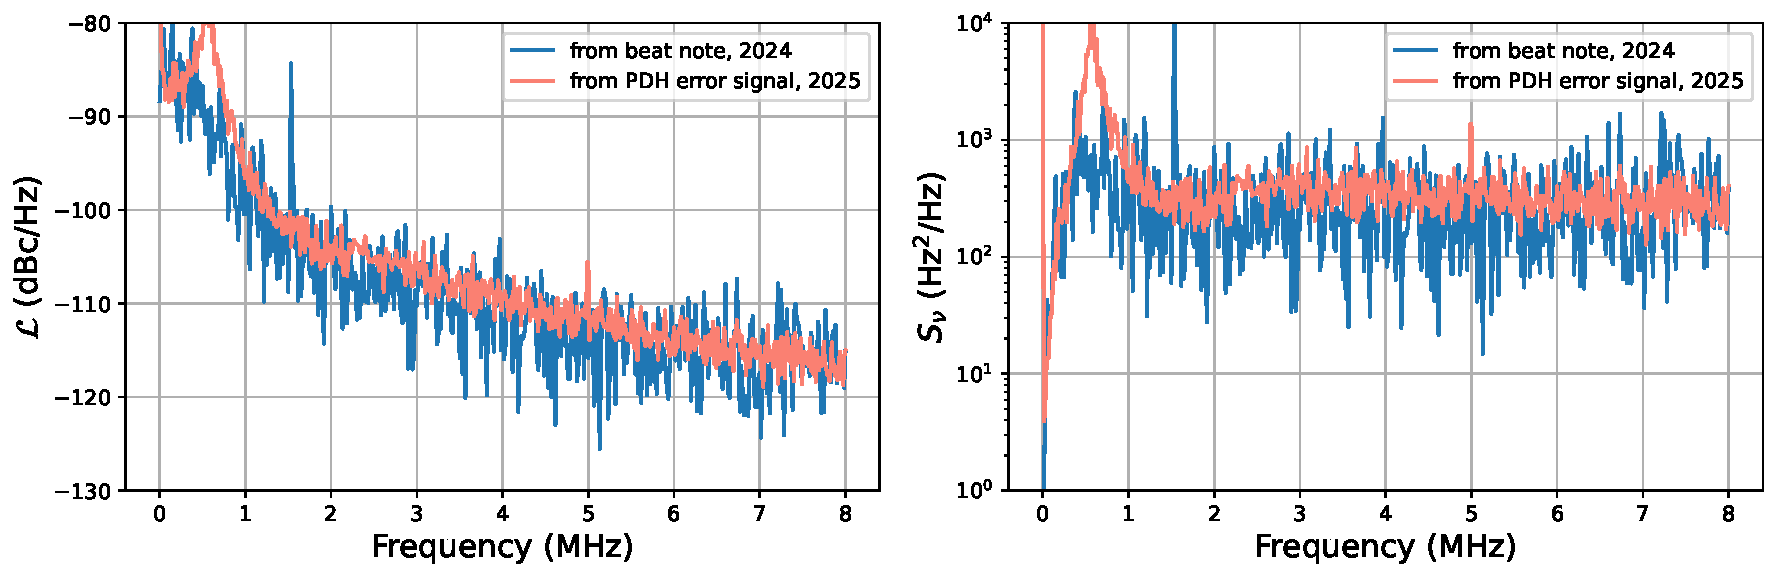
\includegraphics[width=1.0\textwidth]{figures/rydberg/frequency_phase_noise.pdf}
    \caption{\justifying
    \textbf{Frequency and phase noise measurements of the 840 Precilaser fiber amplifier system with two distinct methods.} The left plot displays single sideband phase noise $\mathcal{L}$ in dBc/Hz, and the right plot displays the single-sided frequency noise PSD $S_\nu$. Both quantities are measured by two different methods: the blue curve represents results from the beat note method in 2024, and the red curve represents results from the PDH in-loop error signal method in 2025. Both methods yield consistent results up to servo bump discrepancy, which can be attributed to different locking parameters.
    }
\label{fig:frequency_phase_noise}
\end{figure}

\subsubsection{Method Comparison}
The phase and frequency noise measurement results from both methods are plotted in Figure~\ref{fig:frequency_phase_noise}.  The two methods yield consistent results. 

\subsection{Gate Fidelity Simulation}

Given the measured frequency noise spectrum $S_\nu(f)$, we estimate the phase-noise-limited CZ gate infidelity using the fidelity response theory (FRT) developed by Tsai et al. \cite{Tsai2025}. The central idea of FRT is that when the noise is a small perturbation to the driving Hamiltonian, the gate infidelity can be expressed as a linear functional of the noise power spectral density weighted by a gate-specific fidelity response function:
\begin{align}
    \varepsilon_\nu = \int_0^\infty df\, S_\nu(f)\, I_\nu(f;\,\Omega), \label{eqn:FRT_integral}
\end{align}
where $S_\nu(f)$ is the single-sided frequency noise PSD of the Rydberg laser and $I_\nu(f;\,\Omega)$ is the frequency-noise fidelity response function at Rydberg Rabi frequency $\Omega$. This formulation cleanly separates the contribution of the laser noise spectrum from the gate protocol: the response function $I_\nu$ encodes all information about the gate pulse shape and the Hilbert space dynamics, while $S_\nu$ encodes the experimental noise environment.

For an ideal time-optimal CZ gate (zero rise and fall time, infinite blockade interaction strength, and no self-light shift), the response function obeys a universal scaling law \cite{Tsai2025}:
\begin{align}
    I_\nu(f;\,\Omega) = \Omega^{-2}\, g_\nu\!\left(\frac{2\pi f}{\Omega}\right), \label{eqn:scaling_law}
\end{align}
where $g_\nu(x)$ is a dimensionless universal response function that depends only on the gate protocol. 


% This scaling has an intuitive interpretation: faster gates (larger $\Omega$) are less sensitive to slow frequency noise because the gate duration $T \propto \Omega^{-1}$ is shorter, giving the noise less time to accumulate phase errors. The $\Omega^{-2}$ prefactor, combined with the observation that the response function is approximately flat up to $f \sim \Omega/2\pi$ and the noise PSD is largely contained within this bandwidth, predicts that the total frequency-noise-induced infidelity scales approximately as $\Omega^{-2}$.

For the fidelity metric $F_\text{sym}$ (averaged over symmetric Haar random states on the two-qubit symmetric subspace), the universal response function (for the ideal time-optimal CZ gate used in the paper) is well approximated by a double-Gaussian fit (Appendix L of Ref.~\cite{Tsai2025}):
\begin{align}
    \frac{g_\nu(x)}{(2\pi)^2} = a\, e^{-\left(\frac{x-b}{c}\right)^2} + d\, e^{-\left(\frac{x-e}{f}\right)^2},
\end{align}
with fit parameters $a = 3.062$, $b = -0.01507$, $c = 0.5588$, $d = 2.843$, $e = 1.232$, $f = 0.5339$.

\begin{figure}[h!]
\centering
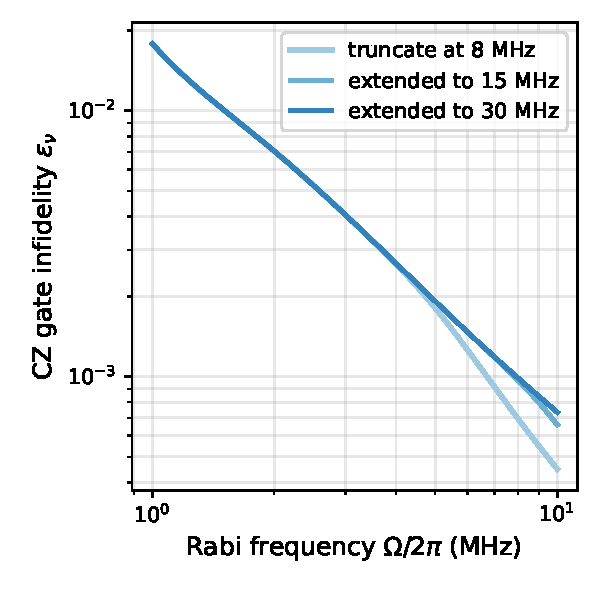
\includegraphics[width=0.6\textwidth]{figures/rydberg/gate_infidelity_cutoff_study.pdf}
    \caption{\justifying
    \textbf{Frequency-noise-limited CZ gate infidelity for different integration bandwidths.}
    Using the fidelity response theory of Tsai et al.\ \cite{Tsai2025}, we compute the time-optimal CZ gate infidelity due to 840~nm laser frequency noise as a function of Rabi frequency. The infidelity is evaluated by numerically integrating Equation~\ref{eqn:FRT_integral}. We first integrate only over the measured frequency-noise PSD, up to 8~MHz, and label this curve ``truncate at 8~MHz.'' We then artificially extrapolate the measured PSD beyond 8~MHz, assuming that it remains flat, and integrate up to 15~MHz or 30~MHz. The three curves overlap for Rabi frequencies below approximately 5~MHz and begin to diverge at larger $\Omega$, where the gate response has appreciable weight at Fourier frequencies beyond the measured 8~MHz window.
    }
\label{fig:gate_fidelity}
\end{figure}

In this simulation, we use the frequency-noise PSD obtained from the PDH error-signal method described in Section~\ref{subsec:phasenoise} as the input $S_\nu(f)$, since this measurement is less noisy than the beat-note-based result. The electronic background noise floor is subtracted in order to isolate the laser frequency noise. Since the 840~nm light is frequency doubled to produce the 420~nm Rydberg excitation beam, the frequency-noise PSD at the atoms is four times the measured 840~nm value: frequency doubling doubles the optical phase and hence doubles the instantaneous frequency fluctuations, while the corresponding PSD scales as the square of this factor. The gate infidelity is then evaluated by numerically integrating Equation~\ref{eqn:FRT_integral} over the specified frequency range while sweeping the Rabi frequency $\Omega/2\pi$ from 1 to 10~MHz, as shown in Figure~\ref{fig:gate_fidelity}.

Because our frequency-noise PSD measurement extends only to 8~MHz, the most direct choice is to integrate Equation~\ref{eqn:FRT_integral} over the measured bandwidth. This is shown as the ``truncate at 8~MHz'' curve in Figure~\ref{fig:gate_fidelity}. However, unlike the spectrum reported by Tsai et al.\ \cite{Tsai2025}, the frequency-noise PSD of our 840~nm laser system does not roll off within the measured range and remains approximately flat up to 8~MHz. Therefore, noise above 8~MHz may contribute non-negligibly to the FRT integral, especially at larger Rabi frequencies (e.g. 10~MHz) where the response function $g_\nu(2\pi f/\Omega)$ is still non-negligible for $f \gtrsim 8$~MHz.

To estimate the possible underestimation caused by the finite measurement bandwidth, we artificially extrapolate the PSD beyond 8~MHz by continuing the observed flat noise floor, and then repeat the integration with upper limits of 15~MHz and 30~MHz. This provides a worst-case estimate of the impact of unmeasured high-frequency noise, assuming that the PSD does not quickly spike up above our measurement window. As shown in Figure~\ref{fig:gate_fidelity}, the additional PSD above 8~MHz has little effect for Rabi frequencies below approximately 5~MHz. At $\Omega/2\pi = 10$~MHz, however, extending the flat PSD to 30~MHz increases the predicted infidelity from approximately 0.04\% to 0.07\%.

These results indicate that the present 840~nm laser system is likely a significant limitation for reaching two-qubit gate fidelities at the 99.9\% level. At a Rabi frequency of 10~MHz, laser frequency noise alone is predicted to contribute approximately 0.04--0.07\% to the CZ gate infidelity, depending on the assumed behavior of the PSD above the measured 8~MHz bandwidth. This contribution already accounts for a substantial fraction of the total error budget allowed for a 99.9\% fidelity target. Consequently, replacing the 1544 nm FECL seed with a lower-noise alternative will likely be necessary to surpass the 99.9\% threshold. Nevertheless, for the initial phase of Rydberg experiments of our platform, the current laser phase noise performance may be sufficient, assuming that the immediate research objectives do not pose strict fidelity requirements beyond  99$\sim$99.5\% level. A transition to a higher-performance seed laser should, however, be prioritized for future iterations aiming for state-of-the-art performance.

\bibliographystyle{unsrt}
\bibliography{references}
\end{document}














